%FOR PDFLATEX USE ONLY
\documentclass[a4paper,12pt]{article}

\usepackage{amssymb,amsmath} %math symbols

\usepackage[margin=2cm]{geometry} %paper geometry

\usepackage[T1, T2A]{fontenc}

\usepackage[utf8]{inputenc} %allows unicode (including russian) source file
\usepackage[russian]{babel} %docment in russian-style
\usepackage[utf8]{inputenc}
%\usepackage[unicode]{hyperref} %links inside of the text
\usepackage[pdftex]{graphicx} %includegraphics pictures
\usepackage{cmlgc} %bold text

\usepackage{array} %arrays

%\usepackage{wrapfig}
%\usepackage{array}
%\usepackage{lipsum}
%\usepackage{esvect}
%\usepackage{hyperref}

\usepackage{amsmath}
\usepackage{amssymb}
\usepackage{mathtools}
\usepackage{mathtext}

\usepackage{subfig}
%\usepackage{calc}
%\usepackage{pgfplots,tikz,circuitikz}
%\usepackage{tkz-euclide}
\include{data_40_1}

\begin{document}

\begin{center}
  \LARGE{Работа 2.2.1}\\[0.2cm]
  \LARGE{Исследование взаимной диффузии газов}\\[0.2cm]
  \large{Стрижак Даниил}\\[0.2cm]
\end{center}  
  
\section{Аннотация}
В данной работе регистрируется зависимость концентрации гелия в воздухе от времени с помощью датчиков теплопроводности при разных начальных давлениях смеси газов, а так же определяется коэффициент диффузии по результатам измерений.

\section{Теоретические сведения}
\textit{Диффузия} -- самопроизвольное взаимное проникновение веществ друг в друга, происходящее вследствие хаотичного теплового движения молекул. При перемешивании молекул разного сорта говорят о \textit{взаимной диффузии}.\\
В системе из двух компонентов зависимость плотности потока компонентов $j_{a,b}$ от их концентрации $n_{a,b}$, подчиняются \textit{закону Фика}:
\begin{equation*}
j_{a,b} = -D\nabla{n_{a,b}}\\
\end{equation*}
В данной работе исследуется взаимная диффузия гелия и воздуха в тонкой трубе. Давление и температура в условиях опыта предполагаются неизменными ($P\ =\ (n_{He}+n_{возд.}) \cdot k_Б; \ \ \ T\ =\ const$), где $n_{He}\ и\ n_{возд.}$ -- концентрации гелия и воздуха соответственно. Поэтому для любых изменений концентрации справедливо $\Delta (n_{He} = - \Delta n_{возд.}$, значит, достаточно ограничиться описанием диффузии одного из компонентов, например для гелия. \\
\begin{equation*}
j_{He} = -D\frac{\partial n_{He}}{\partial x}\\
\end{equation*}
В силу того, что в работе концентрация гелия должна быть мала и из-за того, что атомы гелия существенно легче молекул, составляющих воздух, средняя тепловая скорость частиц гелия велика по сравнению с частицами воздуха, а значит, перемешивание газов в данном эксперименте можно приближенно описывать диффузию примеси легких частиц Не на практически стационарном фоне воздуха. Коэффициент диффузии в таком приближении равен.  \\
\begin{equation*}
D = \frac{1}{3} \lambda \bar{v}; \ \ \ \ \ \bar{v} = \sqrt{\frac{8RT}{\pi \mu}}\\
\end{equation*}
\begin{center}
\begin{minipage}{0.1\textwidth}
  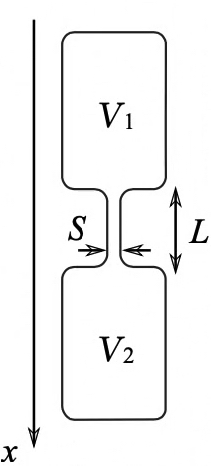
\includegraphics[width=1.5\linewidth]{1.jpg}
\end{minipage}
\begin{minipage}{0.15\textwidth}
\
\end{minipage}
\begin{minipage}{0.7\textwidth}
Для исследования взаимной диффузии газов и измерения коэффициента взаимной диффузии D используется два сосуда объёмами $V_1$ и $V_2$ ($V_1 \approx V_2 = V$), соединенные трубкой длины L и сечения S. Предполагается, что сосуды заполнены смесью двух газов при одинаковом давлении, но с различной концентрацией компонентов. Вследствие взаимной диффузии, проходящей в соединительной трубке, концентрации компонентов в сосудах с течением времени выравниваются.
\end{minipage}
\end{center}
\newpage
Диффузия -- относительно медленный процесс, и для его наблюдения необходимо отсутствие конвекции, т. е. макроскопических течений газа. Для этого необходимо обеспечить равенство давлений и температур в сосудах до начала измерений.\\ 

В данном опыте обьем трубки сильно меньше обьема сосуда, чтобы можно было считать концентрацию компонентов не зависящей от координат.\\

Рассчитаем зависимость концентрации от времени в данном эксперименте:\\
\begin{center}
\begin{minipage}{0.2\textwidth}
\begin{align*}
&j = - D \frac{\partial n}{\partial x} = const \ \ \ \Rightarrow& \\
&\frac{dN_1}{dt} = jS,& \\
&\tau = \frac{VL}{2SD}&\\
\end{align*}
\end{minipage}
\begin{minipage}{0.2\textwidth}
\begin{align*}
&n(x) = \frac{\Delta n}{L} x \ \ \ \Rightarrow&\\
&\frac{dN_2}{dt} = -jS \ \ \ \ \Rightarrow&\\
&\Delta n = \Delta n_0 e^{-\frac{t}{\tau}}&\\
\end{align*}
\end{minipage}
\begin{minipage}{0.2\textwidth}
\begin{align*}
&j = - D \frac{\Delta n}{L}&\\
&\frac{d(\Delta n)}{dt} = -\frac{\Delta n}{\tau}&\\
&\tau \sim \frac{L^2}{2D}&\\
\end{align*}
\end{minipage}
\end{center}
\section{Метод измерений}
Для измерения разности концентраций в установке применяются датчики теплопроводности. При этом используется тот факт, что теплопроводность смеси зависит от её состава. В общем случае зависимость довольно сложна, однако при малой разности концентраций в сосудах можно ожидать, что разность теплопроводностей будет изменяться прямо пропорционально $\Delta n$:
\begin{equation*}
\Delta \kappa = \kappa (n_2) - \kappa (n_1) \approx const \cdot \Delta n\\
\end{equation*}
Эксперименты показывают, что если доля примеси гелия составляет менее 15\%, отклонение от линейной зависимости не превышает 0,5\%, что для наших целей вполне достаточно.\\
Для измерения сопротивлений используется мостовая схема, позволяющая определять разность показаний датчиков с высокой точностью. Мост баллансируется при заполнении сосудов одной и той же смесью. При заполнении сосудов смесями различного состава возникает «дизбаланc» моста. При незначительном различии в составах смесей показания вольтметра, подсоединённого к диагонали моста, будут пропорциональны разности концентраций примеси.\\\
\begin{equation*}
U = U_0 e^{-\frac{t}{\tau}}\\
\end{equation*}
Где $U_0$ -- показание гальванометра в начальный момент времени. Из зависимости напряжения от времени можно получить соответствующее значение коэффициента диффузии. \\
 \newpage
\section{Оборудование и инструментальные погрешности}

\textbf{В работе используются:} измерительная установка; форвакуумный насос; баллон с гелием; манометр; источник питания; магазин сопротивлений; гальванометр; секундомер.\\

\textbf{Инструментальные погрешности измерений:}\\
\begin{itemize}
\item манометр -- 0,5 $кгс/см^2$ \\
\item вольтметр -- 0,1 мВ\\
\item обьем -- $10 \ см^3$\\
\end{itemize}
\begin{center}
ЭКСПЕРИМЕНТАЛЬНАЯ УСТАНОВКА
\end{center}


\begin{center}
\begin{minipage}{0.47\textwidth}
  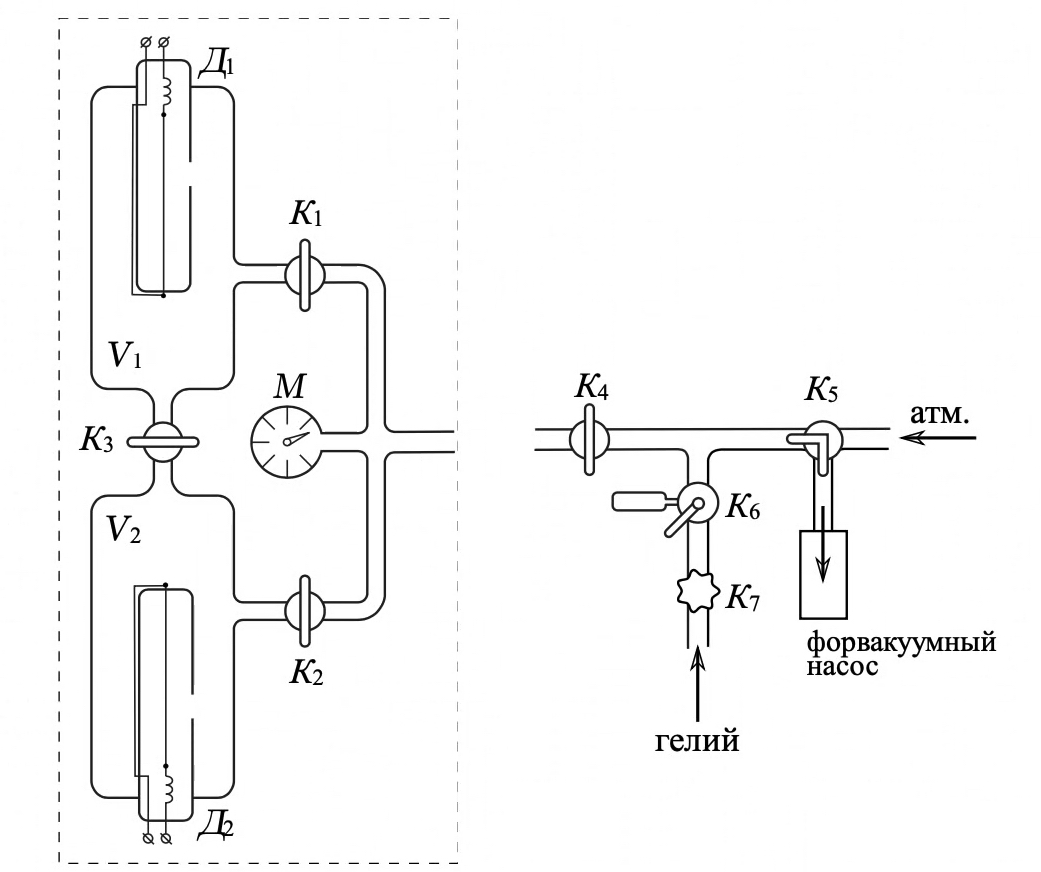
\includegraphics[width=1\linewidth]{2.jpg}
  \begin{center}
  рисунок 1 \ \ \ \ \ \ \ \  рисунок 2
  \end{center}
\end{minipage}
\begin{minipage}{0.04\textwidth}
\
\end{minipage}
\begin{minipage}{0.4\textwidth}
  \begin{center}
 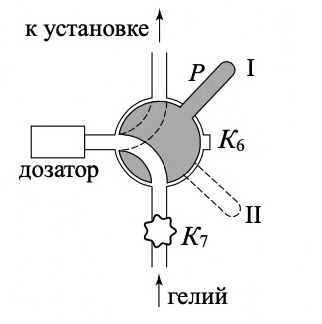
\includegraphics[width=0.5\linewidth]{3.jpg}\\

  рисунок 3
  \end{center}
    \begin{center}
    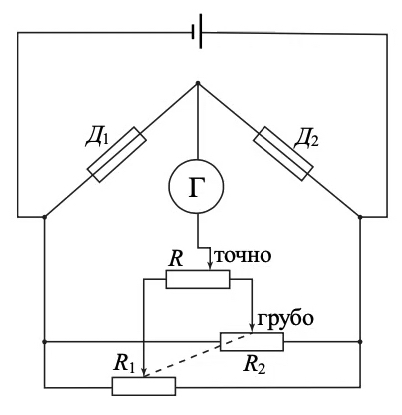
\includegraphics[width=0.5\linewidth]{4.jpg}\\

  рисунок 4
  \end{center}
\end{minipage}
\end{center}

Схема измерительной части установки приведена на рис. 1. Она соединена с системой откачки и напуска воздуха и гелия. Для откачки используется форвакуумный насос. Один из вариантов конструкции изображен на рис. 2. Измерительная часть установки состоит из двух сосудов V1 и V2, размещённых вертикально. Краны К1 и K2 служат для управления откачкой и подачей газа в сосуды. Диффузия осуществляется через тонкую короткую трубку, соединяющую сосуды, оснащённую краном К3. К соединительным трубкам подключен манометр M, измеряющий разность давлений между соединительными трубками и атмосферой. Для подачи малых порций гелия предусмотрен двухходовый кран с дозатором (рис. 3). Датчики теплопроводности Д 1 и Д 2, расположенные в сосудах V 1 и V 2 соответственно, включены в мостовую электрическую схему согласно рис. 5. В одну из диагоналей моста включён высокочувствительный вольтметр Г, к другой подключается источник небольшого постоянного напряжения. Сопротивления проволок датчиков составляют одно из плеч моста. Второе плечо составляют переменные сопротивления R1, R2 и R, служащие для установки показаний вольтметра Г на нуль. Балансировку необходимо проводить перед каждым экспериментом заново: при этом установка заполняется чистым газом при давлении, близком «рабочему».
\section{Результаты измерений и обработка данных}

\subsection{Подготовка к эксперименту}
Ознакомимся с установкой. Согласно руководству:  включим питание электрической схемы, затем очистим установку от всех газов, которые в ней есть. Напустим в установку воздух до рабочего давления чтобы сбалансировать мост на рабочем давлении. Сбалансируем мост. Заполним установку рабочей смесью: в сосуде $V_2$ должен быть воздух, а в сосуде $V_1$ — смесь воздуха, с гелием.\\
Атмосферное давление -- 97.5 кПА, причем минимум давления, откачанный насосом -- 98 $кгс/см^2$, что стоит учесть при рассчете погрешностей. 
\subsection{Проведение измерений}
Проведем измерения после подготовки для разных значений давления. В таблице ниже приведены обработанные результаты измерений. Повторные измерения при 40 и 80 торр производились в обратных пропорциях гелия и воздуха(1,675 частей гелия и 0,2 части воздуха). Центровка в данном случае производилась гелием. Графики, с помощью которых производился рассчет времени релаксации для определенного давления представлены в приложении. Таблицы с измерениями и программный код, обрабатывающий данные, лежат в отдельных файлах в силу своей громоздкости. 

\begin{center}
\begin{tabular}{|c|c|c|c|c|c|}
\hline
 $  No   $ & $  Р, \ кгс/см^2 $ & $Р, \ торр  $ & $  \tau, \ c  $  & $    D, \ см^2/c  $  & $\frac{1}{P}, \ Па^{-1}$ \cdot 10^{-4}\\
\hline 
     1    &       92  &   40  &   192     &     10,7    &  1,87  \\
\hline
    2     &    87     &   80  &   321     &      6,4    &0,94   \\
\hline
    3     &    77     &  154   &    647    &      3,2     &0,49  \\
\hline
      4   &      73,5   &  180   &    767    &      2,7   &   0,42 \\
\hline
        5 &   65      &   240  &   1047     &       2,0   & 0,31  \\
\hline
         6&     92,5    &  40   &     149   &       13,7   & 1,87 \\
\hline
        7 &       87,5  &    80 &   350     &      5,9    &  0,94 \\
\hline
\end{tabular}
\end{center}
Ниже приведена графическая обработка данных, откуда можно найти коэффициент диффузии при атмосферном давлении. 
\begin{center}
\begin{tikzpicture}[scale = 1.3]
\begin{axis}[
    legend style={at={(0.7,0.97)}},
    axis lines = left,
    xlabel = {$P^{-1}, Па^{-1} \cdot 10^{-4}$},
    ylabel = {$D,\ см^2/c$},
    xmin=0, xmax=2,
    ymin=0, ymax=14,
	ymajorgrids = true,
	xmajorgrids = true,
	yminorgrids = true, 
	xminorgrids = true, 
	minor tick num = 4 
]

\addplot+[only marks ] plot[error bars/.cd, y dir=both, y explicit]
  coordinates {
	 (1.87,11.2)+-(1.2,1.2)
	 (1.87, 13.4)+-(1.2,1.2)
	 (0.94, 6.4)+-(0.8,0.8)
	 (0.94, 5.9)+-(0.8,0.8)
	 (0.49, 3.2)+-(0.6,0.6)
	 (0.42, 2.7)+-(0.5,0.5)
	 (0.31, 2)+-(0.4,0.4)};
	

\addplot+[blue] coordinates{(  -1,-6.626 ) ( 5,33.13)};	

	
\legend{ 
	$Зависимость \ D \ от \ \frac{1}{P}$\\
	};

\end{axis}
\end{tikzpicture}
\end{center}
\\
Из графика можно сделать заключение, что зависимость является прямой пропорциональностью с коэффициентом k = 6,6 $\pm 1,0\ \frac{кг\cdotм}{c^3}$, а коэффициент диффузии при атмосферном давлении составляет D = 0,66 $ \pm 0,10\ \frac{см^2}{c}$  при табличном значении D = 0,57 $\frac{см^2}{c}$. \\
Из вычисленного значения коэффициента взаимной диффузии оценим длину свободного пробега атомов гелия в воздухе при нормальных условиях:

\[ \lambda_{He} = 3D \cdot \sqrt{\frac{\pi \mu}{8RT}} = (1,6 \pm 0,2) \cdot 10^{-7} м\]\\

Оценим среднее сечение столкновения частиц гелия с воздухом \[$n_{\Sigma} = n_{He} + n_{air} = P_{\Sigma}/k_B T$, $\sigma = 1/\lambda n_{\Sigma} =1/ 3D \cdot \sqrt{8k_B T / \pi \mu} \cdot k_B T/P_{\Sigma}$: \sigma = (4,3 \pm 0,6) \cdot 10^{-19} м^2 \]



 \section{Выводы и рассчёт погрешностей}
 \subsection{Погрешности}
 \begin{equation*}
\frac{\Delta D}{D} = \sqrt{\frac{1}{N^2}\sum\limits_1^n{((\frac{\Delta V}{V})^2+(\frac{\Delta t}{t})^2})+(\frac{\Delta \frac{L}{S}}{\frac{L}{S}})^2+(\frac{\Delta V}{V})^2+\sigma_{эксп}^2} \approx 14\%
\end{equation*}
\begin{equation*}
\frac{\Delta \lambda_{He}}{\lambda_{He}} =\sqrt{(\frac{\Delta D}{D})^2+\frac{1}{4}(\frac{\Delta T}{T})^2} \approx 14\%
\end{equation*}
\begin{equation*}
\frac{\Delta \sigma}{\sigma} = \sqrt{(\frac{\Delta D}{D})^2+\frac{9}{4}(\frac{\Delta T}{T})^2+(\frac{\Delta P_\Sigma}{P_{\Sigma}})^2} \approx 15\%
\end{equation*}
 \subsection{Вывод}
 В результате эксперимента было получено значение коэффициента диффузии гелия в воздухе, значение длины свободного пробега и среднее значение сечения столкновения частиц гелия с воздухом. Небольшое отклонение, пренебрежимо малое в этой задаче, связано с нагревом воздуха из-за теплообмена с нагретым проводником. В целом, полученные данные совпадают с табличными в пределах погрешности, что говорит о том, что методика эксперимента достаточно хороша и можно оценивать не только порядок. 
\section{Приложение}
\begin{minipage}{0.47\textwidth}
  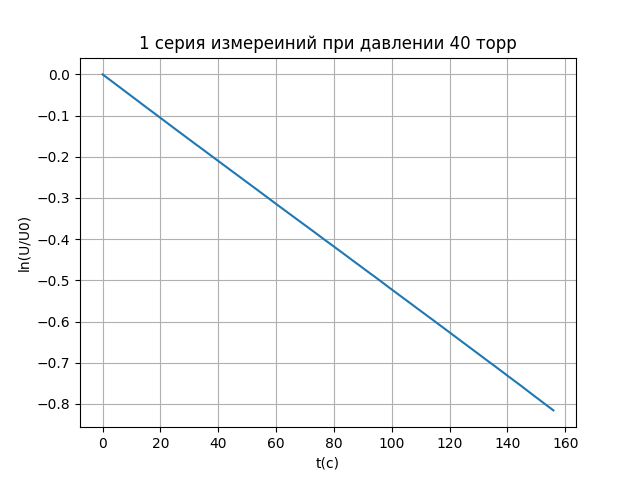
\includegraphics[width=1\linewidth]{pic/40_1.png}
\end{minipage}
\begin{minipage}{0.04\textwidth}
\
\end{minipage}
\begin{minipage}{0.47\textwidth}
 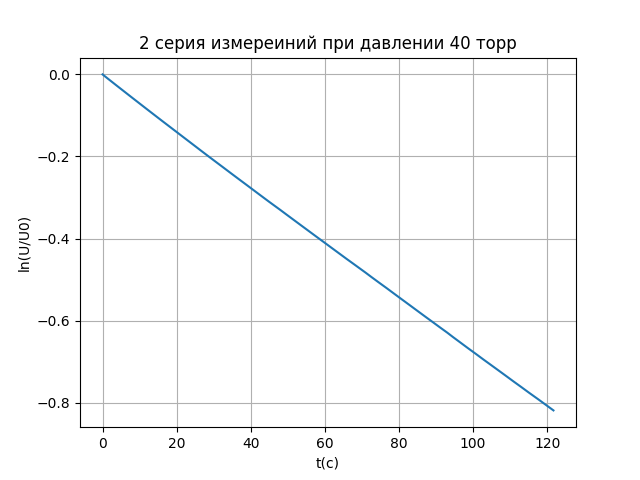
\includegraphics[width=1\linewidth]{pic/40_2.png}
\end{minipage}
\\
\
\\
\\

\
\\
\begin{minipage}{0.47\textwidth}
  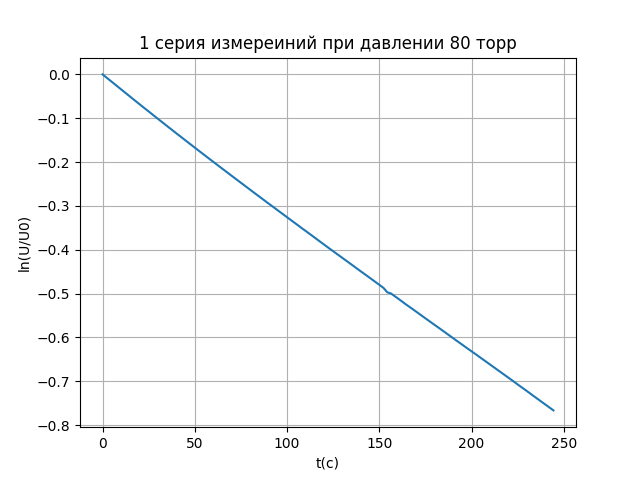
\includegraphics[width=1\linewidth]{pic/80_1.png}
\end{minipage}
\begin{minipage}{0.04\textwidth}
\
\end{minipage}
\begin{minipage}{0.47\textwidth}
 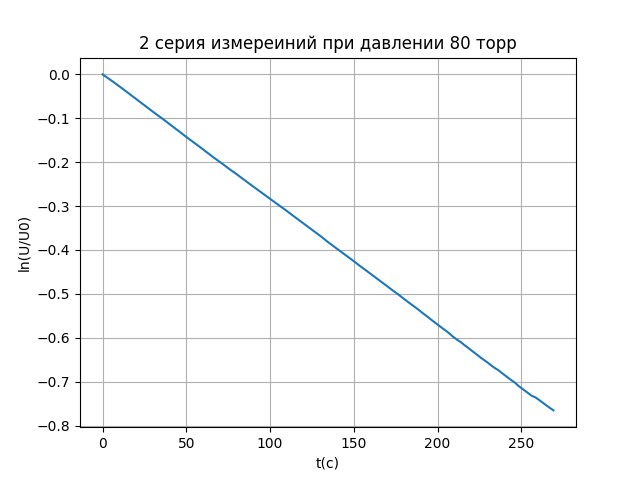
\includegraphics[width=1\linewidth]{pic/80_2.png}
\end{minipage}
\\
\
\\
\\

\
\\
\begin{minipage}{0.47\textwidth}
  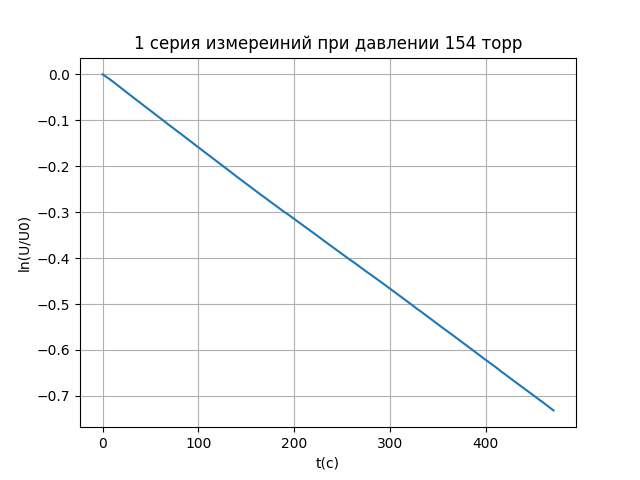
\includegraphics[width=1\linewidth]{pic/154_1.png}
\end{minipage}
\begin{minipage}{0.04\textwidth}
\
\end{minipage}
\begin{minipage}{0.47\textwidth}
 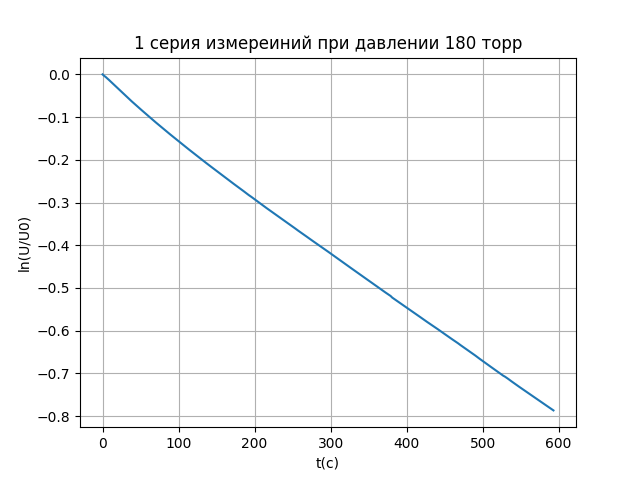
\includegraphics[width=1\linewidth]{pic/180_1.png}
\end{minipage}
\\
\
\\
\\

\
\\
\begin{minipage}{\textwidth}
  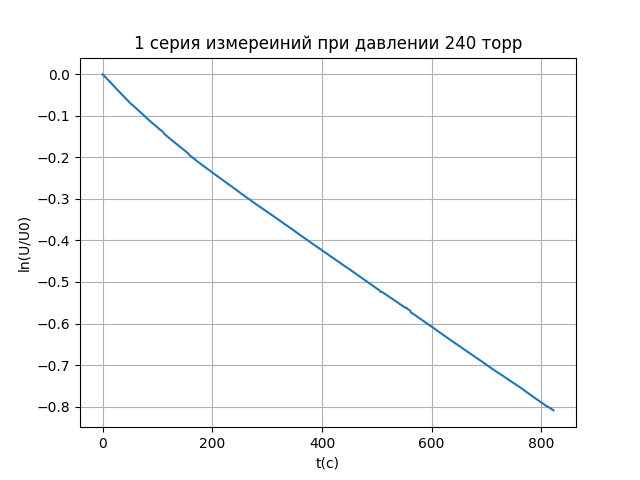
\includegraphics[width=1\linewidth]{pic/240_1.png}
\end{minipage}


\end{document}
